\documentclass{beamer}
\usepackage[utf8]{inputenc}
\usepackage[english]{babel}
\usepackage{listings}
\usepackage{moreverb}
\usepackage{hyperref}
\usepackage{graphicx}
\usetheme{Madrid}
\title[Classifying Laser Range Data "Images"] % (optional, only for long titles)
{Classifying Laser Range Data "Images"}
\subtitle{Supervisor: Elin Anna Topp}
\author[F. Paulsson, S. Senanayake]% (optional, for multiple authors)
{Fredrik Paulsson \and Shan Senanayake}
\institute[LTH] % (optional)
{Lund University \\ Faculty of Engineering}
\date[\today] % (optional)
{\today}
%\subject{Computer Science}
%\setcounter{secnumdepth}{5}
%\setcounter{tocdepth}{5}
\begin{document}
\frame{\titlepage}
%\tableofcontents

\begin{frame}
\frametitle{Project Description}
\framesubtitle{Purpose and Goals}

The main task of the project was to make a robot identify certain elements in its surroundings, for example, doors, chairs, tables, humans, e.t.c.

\vspace{10pt}

Thus we divided the project into three parts:

\begin{itemize}
\pause
\item{Create a parser for the laser range data and transform the data into a more suitable coordinate system}
\pause  
\item{Develop an algorithm that can classify laser range measurements}
\pause  
\item{If time is available, port the programs into ROS (Robot Operating System)}
\end{itemize}
\pause
Offline data to be used during development and if ported into ROS maybe test on online data

\end{frame}

\begin{frame}[fragile]
\frametitle{Laser Range Data}
\framesubtitle{Parser}

The laser scanner took measurements with 4-5 Hz. Each measurement was stored in the following format:
\begin{verbatim}
<unknown> <unknown> <number_of_points> <timestamp_seconds>
<timestamp_microseconds> <unknown> <unknown> <unknown>
<unknown> <unknown> <unknown> <angle_between_points>
<unknown> <unknown> <unknown>
<distance_in_meters>^(number_of_points)
\end{verbatim}

1 measurement = 1 line
\\
1 round of measurements = 1 file

\pause
\vspace{10pt}

The parser yields polar coordinates which are hard to work with.

\end{frame}

\begin{frame}
\frametitle{Laser Range Data}
\framesubtitle{Transformation}

When we have parsed the measurements we transform the data from polar coordinates to our own cartesian-coordinates.

\pause
\vspace{10pt}

The robot is located at (0,0) and the robot forward is along the y-axis.

\pause
\vspace{10pt}

Having this coordinate-system makes it much easier to plot the data for us to visually analyze the measurements as well as to process the data.

\pause
\vspace{10pt}

For instance, we can use well-known algorithms and mathematical formulas to interpolate the data or find patterns in the data.


\end{frame}

\begin{frame}
\frametitle{Laser Range Data}
\framesubtitle{Example Plots}

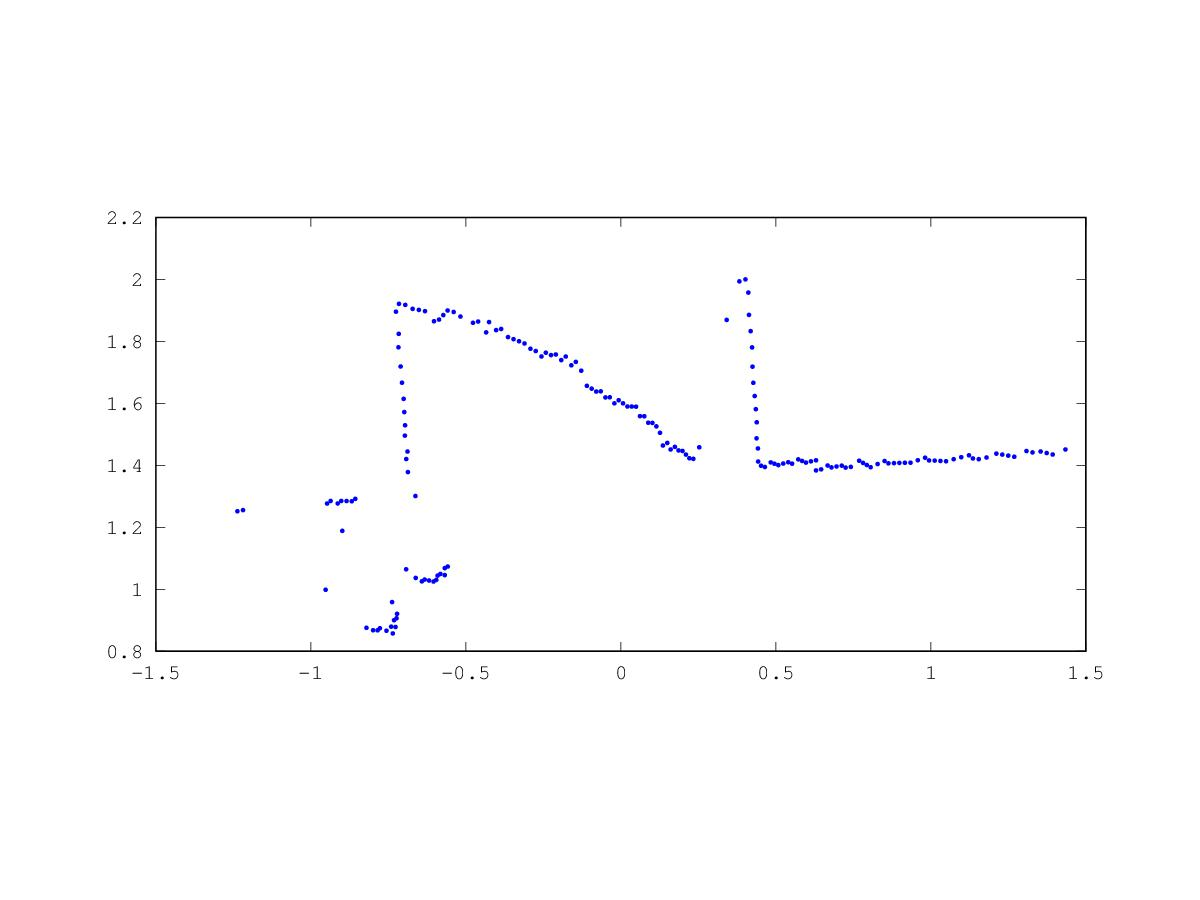
\includegraphics[scale=0.25]{presimg/doorhalf.jpg}
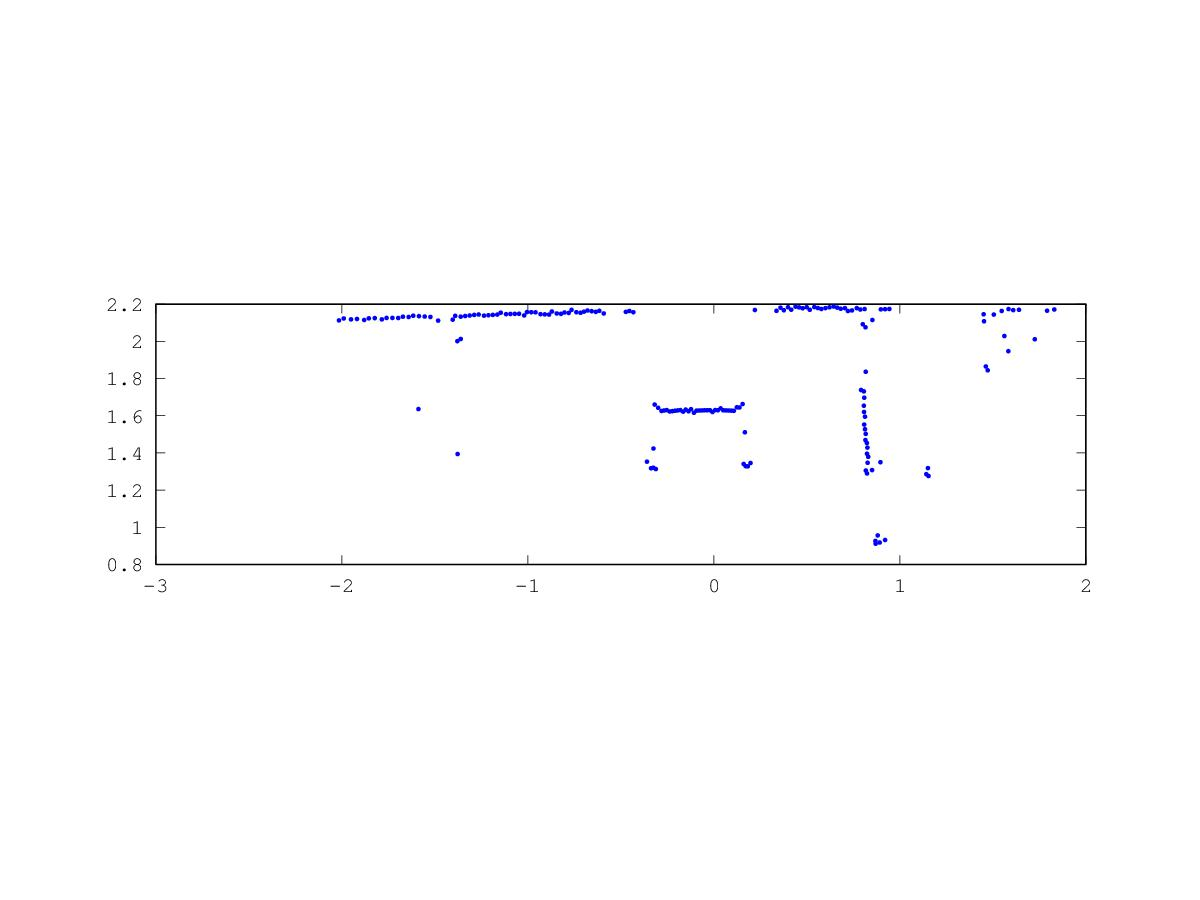
\includegraphics[scale=0.25]{presimg/chair.jpg}

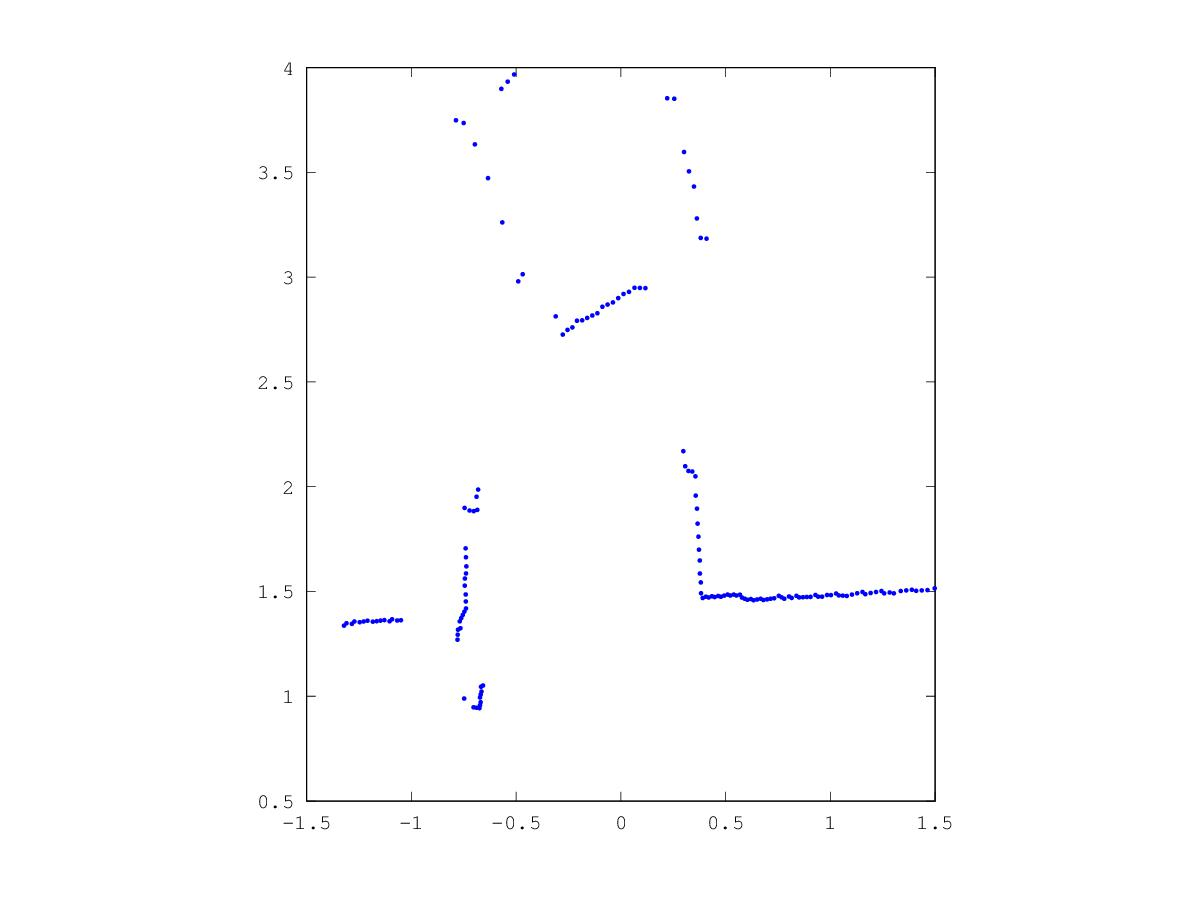
\includegraphics[scale=0.25]{presimg/doorfull.jpg}
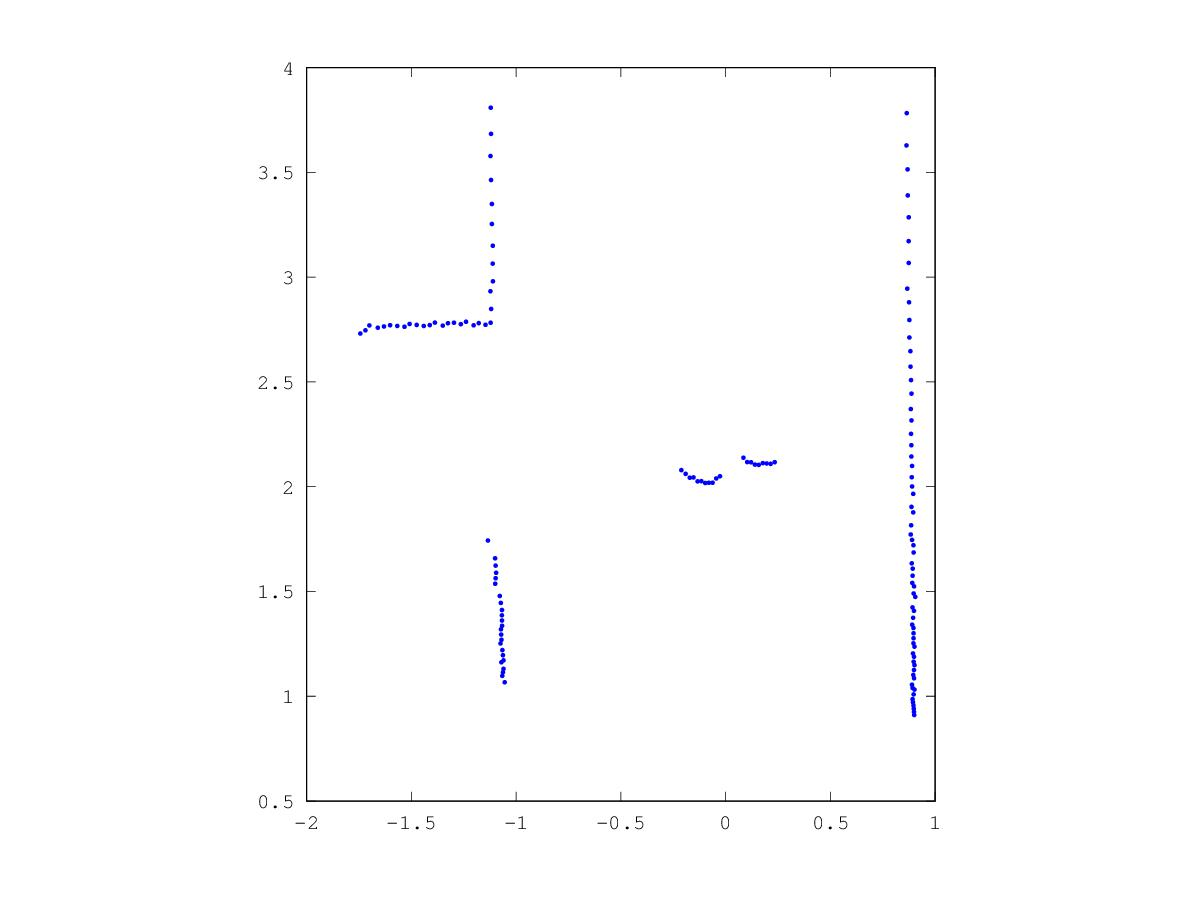
\includegraphics[scale=0.25]{presimg/human.jpg}


\end{frame}


\begin{frame}
\frametitle{Algorithm}
\framesubtitle{Approach}

We are both very interested in the Machine Learning division of Artificial Intelligence.

\pause
\vspace{10pt}

Therefore, our original vision was to try to implement the classifier using unsupervised learning. Thereby letting the classifier improve itself.

\pause
\vspace{10pt}

However, we eventually realized that we needed to use supervised learning in order to have a starting ground.


\pause
\vspace{10pt}

Eventually we had to only use supervised learning as we had to change the way the whole classifier was going to work.

\end{frame}

\begin{frame}[shrink]
\frametitle{Algorithm}
\framesubtitle{Directly Comparing Measurements}

The first approach that we tried to implement was the following:

\begin{itemize}
\pause
\item{Maintaining a list of measurements and their classifications}
\pause
\item{Have some kind of algorithm that directly compares two measurements}
\pause
\item{Using the above algorithm to find the best match in the maintained list}
\pause
\item{Assign the same classification of the best match to the new measurement}
\pause
\item{Add our newly classified measurement to the list}
\end{itemize}

\pause
This approach combines supervised and unsupervised learning. We must have a starting list, this is supervised learning, and as the list grows we have unsupervised learning.

\pause
\vspace{10pt}

However, this approach has some problems.

\begin{itemize}
\pause
\item{Difficult to find an algortihm to compare measurements}
\pause
\item{Since the list grows, the classifier can introduce small errors that will accumulate}
\end{itemize}

\end{frame}

\begin{frame}
\frametitle{Algorithm}
\framesubtitle{Directly Comparing Measurements}

The simple interpolation-algorithm to do comparisons:

\begin{itemize}
\pause
\item{Draw even lines between all the points in a dataset}
\pause
\item{Output a new dataset consisting of evenly distributed points in a dataset}
\end{itemize}

\pause
However this is quite an unstable solution since slightest shift will become an error.


\end{frame}

\begin{frame}
\frametitle{Algorithm}
\framesubtitle{Line Finding}

The next approach was to go up a abstraction level and try to locate intresting characteristics of the data set.
Which led us to the line finding algorithm.
\pause

\begin{equation} \label{eq1}
\begin{split}
y & = kx + m \\
y_{upper}  & =  kx + m + err \\
y_{lower} & = kx + m - err \\
\end{split}
\end{equation}
\begin{enumerate}
\pause
\item{\label{itm:first}Find the first line between startpoint and the next point}
\item{\label{itm:snd}Check if the next point is in bounds of $y_{upper}$ and $y_{lower}$}
\item{If \ref{itm:snd} Adjust the original line with weight to the new point}
\item{When done check if line length $>$ 0.2 m and has at least 3 points}
\item{Repeat \ref{itm:first} until no more points can be checked}
\end{enumerate}


\end{frame}

\begin{frame}
\frametitle{Algorithm}
\framesubtitle{Line Finding}
Ran linefinding with 0.2 m thick line, and 10 degrees of margin of error for finding perpendicular and parallell lines.
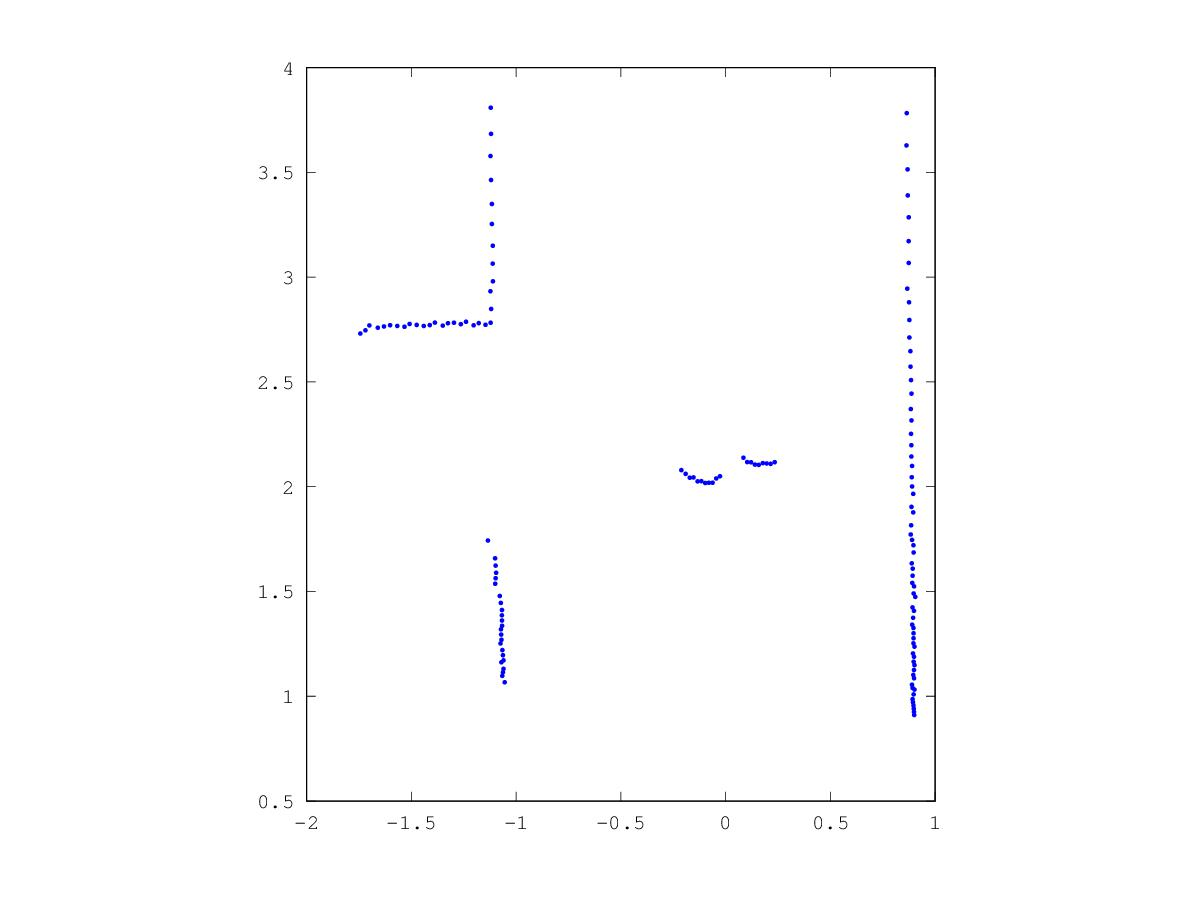
\includegraphics[scale=0.3]{presimg/human.jpg}
\begin{itemize}
\item{Number of lines: 5}
\item{Mean length of lines: 0.892474 m}
\item{Parallell: 4}
\item{Perpendicular: 3}
\end{itemize}


\end{frame}

\begin{frame}
\frametitle{Algorithm}
\framesubtitle{The Decision Tree}

Now that we had a way to represent data we could chose a machine learning algorithm to learn patterns.

\pause

The algorithm we chose was the ID3 (Decision tree algorithm) which was a perfect algorithm to represent this abstract data structure.



\end{frame}

\begin{frame}
\frametitle{Algorithm}
\framesubtitle{The Decision Tree}

Now that we had a way to represent data we could chose a machine learning algorithm to learn patterns.

\pause
\vspace{10pt}

The algorithm we chose was the ID3 (Decision tree algorithm) which was a perfect algorithm to represent this abstract data structure.


\end{frame}

\begin{frame}[fragile]
\frametitle{Algorithm}
\framesubtitle{The Decision Tree}
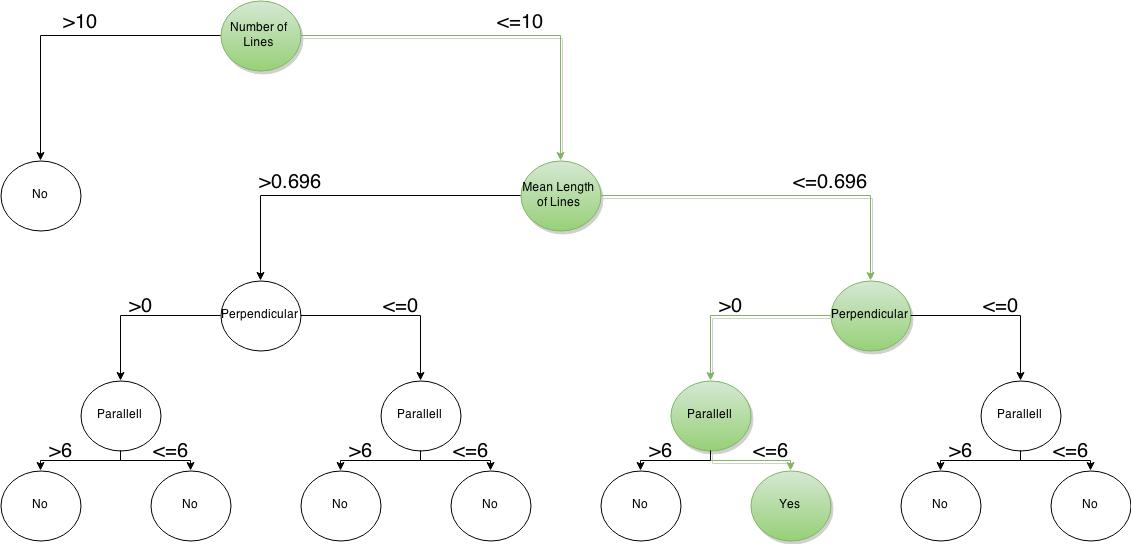
\includegraphics[scale=0.3]{presimg/id3.jpg}

\end{frame}

\begin{frame}
\frametitle{Conclusion}

\end{frame}


\end{document}